% Asal-usul (tidak pernah dicetak): lihat sources/outline_sources.md (Tahun 1: gravitasi dan
% pengukurannya, gravitasi normal; isostasi, Airy dan Pratt; anomali udara-bebas dan Bouguer;
% geoid). Kurva dari figdata/bachelor-1/hypsometry.py dan gravity_profiles.py; nilai soal latihan
% dan soal dihitung dalam kalkulator skrap Buku 3 calc/ch11.py.
\chapter{Isostasi dan anomali gravitasi}\label{ch:b1:isostasy-gravity}

Pada 1840-an para juru ukur yang mengukur busur meridian di India utara menjumpai selisih yang tidak dapat mereka salahkan pada instrumen mereka. Di antara dua stasiun yang berjarak sekitar 370 mil, Kaliana di kaki Himalaya dan Kalianpur jauh di selatan, selisih \omterm{def:b1:spherical-astronomy:geographic}{lintang} yang diperoleh dari triangulasi melampaui selisih yang diperoleh dari bintang sebesar 5.236 detik busur. Tersangka yang jelas adalah pegunungan: tarikannya menarik tali unting ke utara, dan para astronom mengatur instrumen mereka menurut tali unting itu. Pada 1855 John Henry Pratt menghitung tarikan Himalaya dan dataran tinggi di belakangnya, dan mendapatinya seharusnya membuat selisih itu 15.885 detik, lebih dari tiga kali yang teramati. Pegunungan menarik jauh lebih sedikit daripada yang diperlukan massa tampaknya. Pada tahun yang sama George Airy menjawab bahwa \omterm{def:b1:layered-earth:layers}{kerak} mengapung di atas lapisan yang lebih padat seperti rakit kayu di atas air, sehingga tanah tinggi memiliki akar dalam dari batuan ringan; Pratt kemudian mengusulkan jawaban lain, yaitu batuan yang dibuat lebih ringan oleh pemuaian di bawah pegunungan. Keduanya masih diajarkan: pegunungan didasari oleh batuan ringan yang mengimbangi massanya. Bab ini mengubah gagasan itu menjadi angka, dan menunjukkan bagaimana gravitasi, yang diukur hingga sepersejuta nilainya, mengungkapkan massa yang tersembunyi di bawah relief.
% ledger: pratt:himalaya, airy:1855, pratt:1871

\begin{recall}
Hukum gravitasi Newton memberikan medan $g = GM/r^2$ di luar massa bola $M$; medan itu berasal dari potensial gravitasi, dan permukaan ekuipotensial selalu tegak lurus terhadap medan (fisika). Dalam fluida diam tekanan bertambah dengan kedalaman sebagai $\mathrm dp/\mathrm dz = \rho g$, dan benda yang mengapung memindahkan fluida seberat dirinya (fisika, Sarjana Tahun ke-1). Di bawah \omterm{def:b1:layered-earth:lithosphere}{litosfer} \omterm{def:b1:layered-earth:lithosphere}{astenosfer} mengalir dalam waktu yang panjang; \omterm{def:b1:layered-earth:layers}{kerak} lebih ringan daripada \omterm{def:b1:layered-earth:layers}{mantel} di bawahnya (\cref{ch:b1:layered-earth}; Buku 2, kelas 11).
\end{recall}

\section{Gravitasi dan pengukurannya}

Percepatan gravitasi di permukaan Bumi kira-kira \qty{9.8}{m.s^{-2}}, dan variasi yang menarik bagi ahli geologi sejuta kali lebih kecil. Variasi itu dihitung dalam satuan sistem sentimeter-gram lama, yaitu gal: $\qty{1}{Gal} = \qty{1}{cm.s^{-2}} = \qty{0.01}{m.s^{-2}}$, sehingga
\[
  \qty{1}{\milli\gal} = \qty{e-5}{m.s^{-2}} \approx \num{e-6}\,g .
\]
% ledger: nist:gal
Instrumen lapangan mengukur beberapa perseribu miligal; anomali yang dipelajari dalam bab ini berkisar dari sebagian kecil miligal di atas tubuh bijih yang terkubur hingga beberapa ratus miligal di atas pegunungan.

Bahkan di Bumi yang tanpa relief, gravitasi tidak sama di mana-mana. Bumi berputar, sehingga yang dirasakan tali unting atau gravimeter adalah jumlah tarikan gravitasi dan efek sentrifugal rotasi; dan Bumi gepeng, sehingga kutubnya lebih dekat ke pusatnya daripada ekuatornya. Kedua efek itu membuat gravitasi lebih lemah di ekuator daripada di kutub. Seorang ahli geologi membandingkan setiap pengukuran dengan acuan yang halus yang memuatnya.

\begin{definition}[Gravitasi normal]\label{def:b1:isostasy-gravity:normal-gravity}
\emph{Gravitasi normal}\index{gravitasi normal} $\gamma$ adalah gravitasi dari model Bumi: elipsoid putar dengan massa dan rotasi Bumi, dipilih sehingga permukaannya adalah ekuipotensial dari gravitasinya sendiri (gravitasi ditambah efek sentrifugal). Pada permukaan itu gravitasi normal hanya bergantung pada \omterm{def:b1:spherical-astronomy:geographic}{lintang}.
\end{definition}

Elipsoid itu sendiri, kegepengannya, dan cara parameternya dicocokkan dengan Bumi nyata dipelajari dalam volume Sarjana Tahun ke-3. Di sini kita hanya memerlukan gravitasinya.

\begin{proposition}[Rumus gravitasi normal]\label{prop:b1:isostasy-gravity:normal-formula}
Pada elipsoid acuan yang diadopsi pada 1980, \omterm{def:b1:isostasy-gravity:normal-gravity}{gravitasi normal} pada \omterm{def:b1:spherical-astronomy:geographic}{lintang} geografis $\varphi$ adalah, dalam bentuk deret yang lazim,
\[
  \gamma(\varphi) = \qty{9.780327}{m.s^{-2}}\,\bigl(1 + 0.0053024\sin^2\varphi
  - 0.0000058\sin^2 2\varphi\bigr).
\]
\end{proposition}
\admitted
% ledger: moritz:grs80

Rumus ini memberikan \qty{9.780327}{m.s^{-2}} di ekuator, \qty{9.806200}{m.s^{-2}} pada \ang{45} dan \qty{9.832186}{m.s^{-2}} di kutub: selisih
\qty{5186}{\milli\gal} dari ekuator ke kutub. Rotasi saja menyumbang sebagian besar darinya. Dengan hari sideris \qty{23.9345}{h}, kecepatan sudutnya adalah
$\omega = 2\pi/\qty{86164}{s} = \qty{7.292e-5}{rad.s^{-1}}$, dan percepatan sentrifugal di ekuator, $\omega^2 a$ dengan $a = \qty{6378.137}{km}$, adalah
\qty{0.0339}{m.s^{-2}}, atau \qty{3392}{\milli\gal}; kegepengan memasok sisanya (\cref{exo:b1:isostasy-gravity:2}).
% ledger: earth:Trot, earth:Req, earth:geq, earth:gpole

Gravitasi diukur dengan dua cara. Gravimeter \emph{absolut} menjatuhkan massa uji dalam ruang vakum dan mengikuti jatuh bebasnya dengan interferometer laser, diukur waktunya oleh jam atom: percepatan langsung diperoleh dari jarak dan waktu. Gravimeter \emph{relatif} adalah massa yang digantung pada pegas, yang peregangannya berubah mengikuti gravitasi; ia ringan dan cepat, tetapi hanya memberi selisih antara tempat-tempat, dan ia melayang, sehingga survei kembali ke stasiun dasar yang gravitasinya diketahui. Instrumen absolut terbaik akurat hingga sekitar satu mikrogal, yaitu satu per miliar dari $g$.
% ledger: ngs:absolute-gravity

\begin{inthefield}[Survei gravitasi di darat]
\begin{minipage}[t]{0.55\linewidth}\vspace{0pt}
Survei gravitasi adalah perjalanan pelan dari stasiun ke stasiun. Di setiap stasiun ahli geofisika memasang gravimeter relatif di atas tripodnya, meratakannya, menunggu pegas tenang dan mengambil beberapa pembacaan; penerima penentuan posisi satelit di sampingnya mencatat posisi dan ketinggian stasiun itu. Setiap beberapa jam tim kembali ke stasiun dasar, sehingga penyimpangan pegas dapat diukur dan dihilangkan. Ketinggian sama pentingnya dengan gravitasi: seperti dijelaskan bagian berikutnya, gravitasi turun \qty{0.3086}{\milli\gal} untuk setiap meter ketinggian, sehingga ketinggian yang keliru sebesar \qty{1}{cm} merusak pembacaan sebesar \qty{3}{\micro\gal}. % ledger: usgs73:reduction
\end{minipage}\hfill
\begin{minipage}[t]{0.42\linewidth}\vspace{0pt}
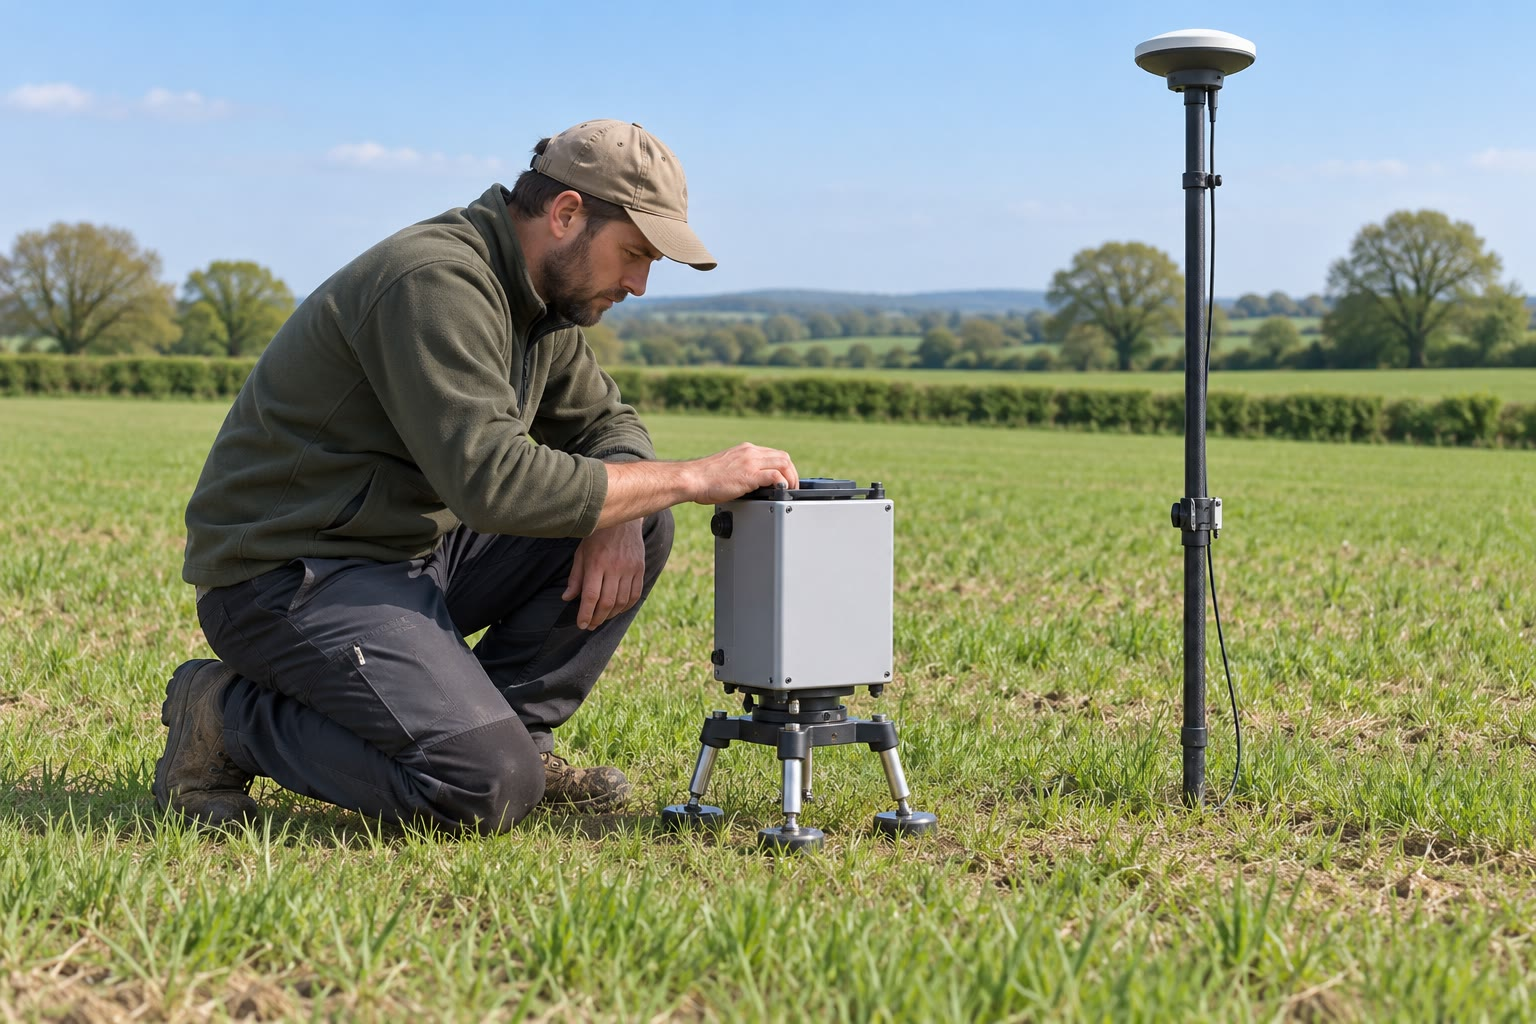
\includegraphics[width=\linewidth]{images/book3/ai/b1-gravity-survey.jpg}

{\scriptsize Gravimeter lapangan di atas tripodnya, dengan antena penentuan posisi satelit di sampingnya (ilustrasi buatan AI).}
\end{minipage}
\end{inthefield}

\section{Isostasi}

Kompensasi yang dibayangkan Airy dan Pratt untuk Himalaya adalah contoh dari keadaan umum lapisan terluar Bumi.

\begin{definition}[Isostasi; kedalaman kompensasi]\label{def:b1:isostasy-gravity:isostasy}
Suatu wilayah berada dalam \emph{isostasi}\index{isostasi}, atau kesetimbangan isostatik, ketika ada suatu kedalaman, \emph{kedalaman kompensasi}\index{kedalaman kompensasi}, tempat tekanannya sama di setiap titik permukaan horizontal, apa pun relief di atasnya. Di bawah kedalaman kompensasi batuan berperilaku sebagai fluida diam; di atasnya, kolom-kolom \omterm{def:b1:layered-earth:layers}{kerak} dan \omterm{def:b1:layered-earth:layers}{mantel} mengapung di atasnya.
\end{definition}

\begin{proposition}[Massa yang sama di atas kedalaman kompensasi]\label{prop:b1:isostasy-gravity:equal-mass}
Jika gravitasi $g$ sama di sepanjang semua kolom, suatu wilayah berada dalam \omterm{def:b1:isostasy-gravity:isostasy}{isostasi} dengan \omterm{def:b1:isostasy-gravity:isostasy}{kedalaman kompensasi} $z_c$ jika dan hanya jika setiap kolom vertikal dengan penampang satuan, dari permukaan hingga $z_c$, memuat massa yang sama.
\end{proposition}

\begin{proof}
Di setiap kolom batuan berada dalam kesetimbangan hidrostatik, sehingga $\mathrm dp/\mathrm dz = \rho(z)\,g$, dengan kedalaman $z$ dihitung ke bawah. Tekanan di permukaan adalah atmosfer, sama di mana-mana (dan dapat diabaikan). Mengintegralkan dari permukaan $z_s$ kolom ke bawah hingga $z_c$ memberikan
\[
  p(z_c) = p_0 + g\int_{z_s}^{z_c}\rho(z)\,\mathrm dz ,
\]
dengan integral adalah massa kolom per satuan luas. Tekanan di $z_c$ sama jika dan hanya jika massa-massa ini sama.
\end{proof}

Dua cara sederhana untuk membagi massa ini menghasilkan dua model klasik (gambar di bawah).

\begin{proposition}[Isostasi Airy]\label{prop:b1:isostasy-gravity:airy}
Misalkan \omterm{def:b1:layered-earth:layers}{kerak} memiliki massa jenis seragam $\rho_c$ dan ketebalan $H$ tempat permukaannya berada di permukaan laut, di atas \omterm{def:b1:layered-earth:layers}{mantel} dengan massa jenis $\rho_m > \rho_c$. Dalam kesetimbangan isostatik:
\begin{enumerate}
  \item di tempat permukaan berada pada ketinggian $h$ di atas permukaan laut, \omterm{def:b1:layered-earth:layers}{kerak} memiliki akar dengan kedalaman $r = h\,\rho_c/(\rho_m - \rho_c)$ di bawah \omterm{def:b1:layered-earth:layers}{kerak} normal,
        dan ketebalan $H + h + r$;
  \item di tempat permukaan berada pada kedalaman $d$ di bawah permukaan laut, di bawah air dengan massa jenis $\rho_w$, \omterm{def:b1:layered-earth:layers}{kerak} memiliki anti-akar: dasarnya terangkat sebesar
        $r' = d\,(\rho_c - \rho_w)/(\rho_m - \rho_c)$, dan ketebalannya adalah
        $H - d - r'$.
\end{enumerate}
Inilah \emph{isostasi Airy}\index{isostasi Airy}: kompensasi oleh perubahan ketebalan pada massa jenis tetap.
\end{proposition}

\begin{proof}
Ambil \omterm{def:b1:isostasy-gravity:isostasy}{kedalaman kompensasi} tepat di bawah akar terdalam, dan bandingkan setiap kolom dengan kolom normal. (1) Kolom tinggi memiliki \omterm{def:b1:layered-earth:layers}{kerak} di tempat \omterm{def:b1:layered-earth:layers}{mantel} sepanjang kedalaman $r$, dan \omterm{def:b1:layered-earth:layers}{kerak} sepanjang ketinggian $h$ tempat kolom normal tidak memiliki apa-apa: massa yang sama mensyaratkan $\rho_c(h + r) = \rho_m r$, yaitu
$r(\rho_m - \rho_c) = \rho_c h$. (2) Kolom rendah memiliki air di tempat \omterm{def:b1:layered-earth:layers}{kerak} sepanjang kedalaman $d$, dan \omterm{def:b1:layered-earth:layers}{mantel} di tempat \omterm{def:b1:layered-earth:layers}{kerak} sepanjang $r'$: massa yang sama mensyaratkan
$\rho_w d + \rho_m r' = \rho_c(d + r')$, yaitu $r'(\rho_m - \rho_c) =
d(\rho_c - \rho_w)$.
\end{proof}

\begin{proposition}[Isostasi Pratt]\label{prop:b1:isostasy-gravity:pratt}
Misalkan setiap kolom berakhir pada \omterm{def:b1:isostasy-gravity:isostasy}{kedalaman kompensasi} yang sama $D$ di bawah permukaan laut, dengan massa jenis seragam di setiap kolom, $\rho_0$ tempat permukaannya berada di permukaan laut. Dalam kesetimbangan isostatik sebuah kolom yang permukaannya berada pada ketinggian $h$ memiliki massa jenis
\[
  \rho(h) = \rho_0\,\frac{D}{D + h},
\]
dan kolom di bawah kedalaman air $d$ memiliki massa jenis
$\rho = (\rho_0 D - \rho_w d)/(D - d)$. Inilah \emph{isostasi Pratt}\index{isostasi Pratt}: kompensasi oleh perubahan massa jenis pada kedalaman tetap.
\end{proposition}

\begin{proof}
Massa yang sama di atas $D$: $\rho(h)(D + h) = \rho_0 D$ untuk kolom tinggi, dan
$\rho_w d + \rho(D - d) = \rho_0 D$ untuk kolom rendah.
\end{proof}

Dengan $\rho_c = \qty{2700}{kg.m^{-3}}$ dan $\rho_m = \qty{3300}{kg.m^{-3}}$, akar Airy adalah $h\times2700/600 = 4.5\,h$: pegunungan setinggi \qty{2}{km} memiliki akar sebesar \qty{9}{km}, dataran tinggi setinggi \qty{4}{km} berakar \qty{18}{km}. Dalam model Pratt dengan $D = \qty{100}{km}$ dan $\rho_0 = \qty{2700}{kg.m^{-3}}$, kedua kolom yang sama memiliki massa jenis 2647 dan \qty{2596}{kg.m^{-3}}, dua dan empat persen lebih ringan. Kedua model menyeimbangkan massa yang sama; keduanya berbeda dalam tempat batuan ringan itu berada, dan itu sesuatu yang dapat dilihat oleh seismologi: Airy memprediksi \omterm{def:b1:layered-earth:discontinuity}{Moho} yang menjadi lebih dalam di bawah pegunungan, Pratt memprediksi \omterm{def:b1:layered-earth:discontinuity}{Moho} yang datar.

\begin{omfigure}
\begin{tikzpicture}[x=0.55cm, y=0.05cm, font=\scriptsize]
% columns computed in calc/ch11.py: Airy roots 9 and 18 km, Pratt densities 2647 and 2596 kg/m3;
% heights above sea level drawn five times larger than depths
\begin{scope}
  \node[font=\small] at (4.5,30) {(a) Airy};
  \fill[omLithGranite!45] (0,0) rectangle (3,-35);
  \fill[omLithGranite!45] (3,10) rectangle (6,-44);
  \fill[omLithGranite!45] (6,20) rectangle (9,-53);
  \fill[omLithPeridotite!45] (0,-35) rectangle (3,-60);
  \fill[omLithPeridotite!45] (3,-44) rectangle (6,-60);
  \fill[omLithPeridotite!45] (6,-53) rectangle (9,-60);
  \draw (0,-60) -- (0,0) -- (3,0) -- (3,10) -- (6,10) -- (6,20) -- (9,20) -- (9,-60);
  \draw (3,0) -- (3,-60) (6,10) -- (6,-60);
  \draw[thick] (0,-35) -- (3,-35) -- (3,-44) -- (6,-44) -- (6,-53) -- (9,-53);
  \draw[densely dashed] (-0.3,-60) -- (9.3,-60);
  \draw[black!50, densely dotted] (-0.3,0) -- (0,0);
  \node[anchor=east] at (-0.3,0) {permukaan laut};
  \node[anchor=east] at (-0.3,-35) {35};
  \node[anchor=east] at (-0.3,-60) {60 km};
  \node at (1.5,-17) {2700}; \node at (4.5,-20) {2700}; \node at (7.5,-24) {2700};
  \node at (1.5,-50) {3300};
  \node[anchor=south] at (1.5,0) {$h = 0$};
  \node[anchor=south] at (4.5,10) {$h = 2$};
  \node[anchor=south] at (7.5,20) {$h = 4$};
  \draw[black!45, densely dotted] (3,-35) -- (9,-35);
  \node at (4.5,-39.5) {akar 9};
  \node at (7.5,-44) {akar 18};
\end{scope}
\begin{scope}[xshift=7.9cm]
  \node[font=\small] at (4.5,30) {(b) Pratt};
  \fill[omLithGranite!45] (0,0) rectangle (3,-100);
  \fill[omLithGranite!36] (3,10) rectangle (6,-100);
  \fill[omLithGranite!27] (6,20) rectangle (9,-100);
  \draw (0,-100) -- (0,0) -- (3,0) -- (3,10) -- (6,10) -- (6,20) -- (9,20) -- (9,-100);
  \draw (3,0) -- (3,-100) (6,10) -- (6,-100);
  \draw[densely dashed] (-0.3,-100) -- (9.3,-100);
  \draw[black!50, densely dotted] (-0.3,0) -- (0,0);
  \node[anchor=east] at (-0.3,0) {permukaan laut};
  \node[anchor=east] at (-0.3,-100) {$D = 100$ km};
  \node at (1.5,-50) {2700}; \node at (4.5,-50) {2647}; \node at (7.5,-50) {2596};
  \node[anchor=south] at (1.5,0) {$h = 0$};
  \node[anchor=south] at (4.5,10) {$h = 2$};
  \node[anchor=south] at (7.5,20) {$h = 4$};
\end{scope}
\end{tikzpicture}

\par\smallskip{\small Dua model klasik \omterm{def:b1:isostasy-gravity:isostasy}{isostasi}, untuk tiga kolom yang berdiri 0, 2 dan \qty{4}{km} di atas permukaan laut (ketinggian dilebih-lebihkan lima kali dibanding kedalaman; massa jenis dalam \unit{kg.m^{-3}}). (a) Airy: satu massa jenis \omterm{def:b1:layered-earth:layers}{kerak}, akar 4.5 kali ketinggian. (b) Pratt: satu \omterm{def:b1:isostasy-gravity:isostasy}{kedalaman kompensasi}, kolom yang lebih ringan di bawah tanah yang lebih tinggi. Setiap kolom membawa massa per satuan luas yang sama di atas \omterm{def:b1:isostasy-gravity:isostasy}{kedalaman kompensasi} yang putus-putus.}
\label{fig:b1:isostasy-gravity:models}
\end{omfigure}

\omterm{def:b1:isostasy-gravity:isostasy}{Isostasi} adalah pernyataan tentang wilayah luas dalam waktu yang panjang. \omterm{def:b1:layered-earth:lithosphere}{Astenosfer} hanya mengalah pada beban yang bertahan selama ribuan tahun, dan \omterm{def:b1:layered-earth:lithosphere}{litosfer} di atasnya cukup kaku untuk menyebarkan beban sempit ke wilayah yang luas dengan melentur, seperti papan membawa beban: sebuah gunung api tunggal tidak perlu dikompensasi di bawahnya sendiri; lenturan \omterm{def:b1:layered-earth:lithosphere}{litosfer} ini dipelajari dalam volume Sarjana Tahun ke-3. Di bawah pegunungan besar \omterm{def:b1:layered-earth:layers}{kerak} jauh lebih tebal daripada rata-rata benua, sekitar \qty{30}{km}: gambaran Airy, akar dari \omterm{def:b1:layered-earth:layers}{kerak} ringan, adalah yang lebih dekat untuk pegunungan. Gambaran Pratt, batuan yang lebih ringan pada kedalaman tetap, menjelaskan punggungan tengah samudra, yang menjulang tinggi di atas \omterm{def:b1:layered-earth:layers}{mantel} atas yang dibuat lebih ringan oleh suhunya yang lebih tinggi.
% ledger: usgs:crust-thickness

\subsection*{Dua tingkat Bumi}

\omterm{def:b1:isostasy-gravity:isostasy}{Isostasi} mengatur relief seluruh planet. Distribusinya diringkas oleh satu kurva.

\begin{definition}[Kurva hipsometrik]\label{def:b1:isostasy-gravity:hypsometry}
Kurva \emph{hipsometrik}\index{kurva hipsometrik} suatu planet memberikan, untuk setiap fraksi $f$ dari permukaannya, ketinggian $z(f)$ yang dilampaui tepat oleh fraksi itu. Ini adalah distribusi kumulatif ketinggian, dibaca dari atas.
\end{definition}

Untuk menggambarnya dari model elevasi berkisi, setiap sel kisi harus diberi bobot menurut luasnya. Pada kisi satu derajat \omterm{def:b1:spherical-astronomy:geographic}{lintang} dan \omterm{def:b1:spherical-astronomy:geographic}{bujur}, sel di antara \omterm{def:b1:spherical-astronomy:geographic}{lintang} $\varphi_1$ dan $\varphi_2$ memiliki luas
$R^2\,\Delta\lambda\,(\sin\varphi_2 - \sin\varphi_1)$, yang menyusut ke arah kutub; dijumlahkan atas semua sel, luasnya memberikan tepat $4\pi R^2$. Mengurutkan sel menurut ketinggian dan mengakumulasikan luasnya memberikan kurva pada gambar di bawah. Kurva itu menunjukkan bahwa \qty{70.9}{\percent} permukaan berada di bawah permukaan laut; bahwa ketinggian rata-rata daratan sekitar \qty{0.8}{km} dan kedalaman rata-rata samudra sekitar \qty{3.7}{km}; dan bahwa sebagian besar permukaan termasuk salah satu dari dua tangga datar, paparan benua dekat permukaan laut dan dasar abisal antara sekitar 3.5 dan \qty{6}{km} di bawah, yang dihubungkan oleh penurunan curam.
% computed in figdata/bachelor-1/hypsometry.py (fraction 0.709, land 793 m, ocean 3692 m); ledger: data:etopo1, wss:ocean-cover

Sebuah planet dengan satu jenis \omterm{def:b1:layered-earth:layers}{kerak}, yang reliefnya terangkat dan aus secara acak, akan memiliki satu tingkat, dengan ketinggian yang tersebar di sekitarnya. Bumi memiliki dua, karena ia memiliki dua jenis \omterm{def:b1:layered-earth:layers}{kerak} dalam kesetimbangan isostatik: \omterm{def:b1:layered-earth:layers}{kerak} benua yang tebal dan ringan mengapung tinggi, \omterm{def:b1:layered-earth:layers}{kerak} samudra yang tipis dan padat rendah (Buku 2, kelas 11). \Cref{exo:b1:isostasy-gravity:8} menunjukkan bahwa model Airy dengan satu massa jenis \omterm{def:b1:layered-earth:layers}{kerak} tidak dapat menghasilkan kedua tingkat itu dengan ketebalan \omterm{def:b1:layered-earth:layers}{kerak} yang teramati.

\begin{omfigure}
\begin{tikzpicture}
\begin{axis}[omrecord, width=0.84\linewidth, height=6.4cm, xmin=0, xmax=100, ymin=-11, ymax=9,
  xlabel={fraksi permukaan Bumi yang lebih tinggi (\unit{\percent})},
  ylabel={ketinggian (km)}, xtick={0,10,...,100}, ytick={-10,-8,...,8},
  tick label style={font=\scriptsize}, label style={font=\small}, clip=true]
% computed in figdata/bachelor-1/hypsometry.py; ledger: data:etopo1
\addplot[name path=hyps, very thick, black] table[x=area_pc, y expr=\thisrow{elev}/1000] {figdata/out/bachelor-1-hypsometry-curve.dat};
\path[name path=sea] (axis cs:0,0) -- (axis cs:100,0);
\addplot[omSea!60] fill between[of=hyps and sea, soft clip={domain=29.1:100}];
\addplot[omHypsLandC!80] fill between[of=hyps and sea, soft clip={domain=0:29.1}];
\draw[black!60, densely dotted] (axis cs:0,0) -- (axis cs:100,0);
\draw[black!60, densely dashed] (axis cs:29.1,-11) -- (axis cs:29.1,9);
\draw[omSea!60!black, densely dashed] (axis cs:29.1,-3.692) -- (axis cs:100,-3.692);
\draw[omHypsLandF, densely dashed] (axis cs:0,0.793) -- (axis cs:29.1,0.793);
  \node[font=\scriptsize, anchor=south east] at (axis cs:99,0.1) {permukaan laut};
  \node[font=\scriptsize, anchor=south, align=center] at (axis cs:18,1.0) {ketinggian rata-rata\\daratan \qty{0.79}{km}};
  \node[font=\scriptsize, anchor=north west, align=left] at (axis cs:31,-3.9) {kedalaman rata-rata\\samudra \qty{3.69}{km}};
  \node[font=\scriptsize, anchor=north west, align=left] at (axis cs:30.5,6.5) {daratan: \qty{29.1}{\percent}\\dari permukaan};
  \node[font=\scriptsize, anchor=north, align=center] at (axis cs:17,-0.5) {paparan\\benua};
  \node[font=\scriptsize] at (axis cs:62,-5.2) {dasar abisal};
\end{axis}
\end{tikzpicture}

\par\smallskip{\small \omterm{def:b1:isostasy-gravity:hypsometry}{Kurva hipsometrik} Bumi, dari model relief global ETOPO1 pada satu derajat, setiap sel diberi bobot menurut luasnya (di atas Antartika dan Greenland, puncak es). Dua bentangan hampir datar pada kurva adalah paparan benua dekat permukaan laut dan dasar laut dalam.}
\label{fig:b1:isostasy-gravity:hypsometry}
\end{omfigure}

\section{Anomali gravitasi}

\subsection*{Dua koreksi}

Gravimeter di atas bukit berada lebih jauh dari pusat Bumi daripada yang di permukaan laut, dan berdiri di atas lapisan batuan yang tidak dimiliki yang lain. Kedua efek itu dihitung sebelum pengukuran dibandingkan dengan \omterm{def:b1:isostasy-gravity:normal-gravity}{gravitasi normal}.

\begin{proposition}[Gradien udara-bebas]\label{prop:b1:isostasy-gravity:free-air}
Di luar Bumi bola dengan jari-jari $R$, gravitasi berkurang terhadap ketinggian $h$ dengan laju
\[
  \frac{\mathrm dg}{\mathrm dh} = -\frac{2g}{R}\,;
\]
pada permukaan, $2g/R \approx \qty{3.08e-6}{s^{-2}}$, kira-kira
\qty{0.308}{\milli\gal} per meter.
\end{proposition}

\begin{proof}
$g(r) = GM/r^2$, sehingga $\mathrm dg/\mathrm dr = -2GM/r^3 = -2g(r)/r$; pada $r = R$,
dengan $g = \qty{9.820}{m.s^{-2}}$ dan $R = \qty{6371}{km}$, $2g/R =
\qty{3.083e-6}{s^{-2}}$.
\end{proof}
% ledger: earth:gmean, earth:Rmean

Perataan dan rotasi mengubah gradien sedikit; nilai yang dipakai dalam praktik ialah sekitar \qty{0.3086}{\milli\gal.m^{-1}}.
% ledger: usgs73:reduction

\begin{proposition}[Lempeng Bouguer]\label{prop:b1:isostasy-gravity:slab}
Lempeng horizontal tak hingga dengan ketebalan $h$ dan massa jenis seragam $\rho$ menarik titik di luarnya dengan percepatan vertikal
\[
  g_B = 2\pi G\rho h ,
\]
apa pun jarak dari titik ke lempeng. Secara numerik $2\pi G =
\qty{0.0419}{\milli\gal}$ per meter ketebalan per \qty{1000}{kg.m^{-3}} massa jenis.
\end{proposition}

\begin{proof}
Letakkan titik di titik asal dan potong lempeng menjadi cincin tipis yang koaksial dengan vertikal melaluinya. Sebuah cincin pada jarak $z$ di bawah titik, dengan jari-jari
$s$, lebar $\mathrm ds$ dan tebal $\mathrm dz$, memiliki massa
$\rho\,2\pi s\,\mathrm ds\,\mathrm dz$, semuanya pada jarak $\sqrt{s^2 + z^2}$;
oleh simetri tarikannya vertikal, sama dengan tarikan setiap elemen
dikali kosinus $z/\sqrt{s^2+z^2}$ dari sudutnya terhadap vertikal:
\[
  \mathrm dg = G\,\frac{\rho\,2\pi s\,\mathrm ds\,\mathrm dz}{s^2 + z^2}\,
  \frac{z}{\sqrt{s^2 + z^2}} .
\]
Untuk satu lapisan, $\int_0^\infty s\,(s^2 + z^2)^{-3/2}\,\mathrm ds =
\bigl[-(s^2 + z^2)^{-1/2}\bigr]_0^\infty = 1/z$, sehingga lapisan menarik dengan
$2\pi G\rho\,\mathrm dz$, tidak bergantung pada $z$. Menjumlahkan lapisan-lapisan sepanjang
ketebalan $h$ memberikan $2\pi G\rho h$. Dengan $G = \qty{6.674e-11}{m^3.kg^{-1}.s^{-2}}$,
$2\pi G\times\qty{1000}{kg.m^{-3}}\times\qty{1}{m} = \qty{4.19e-7}{m.s^{-2}} =
\qty{0.0419}{\milli\gal}$.
\end{proof}
% ledger: const:G

\begin{definition}[Anomali gravitasi]\label{def:b1:isostasy-gravity:anomalies}
Misalkan $g$ gravitasi yang diukur di sebuah stasiun dengan \omterm{def:b1:spherical-astronomy:geographic}{lintang} $\varphi$ dan ketinggian $h$
di atas permukaan laut.
\begin{itemize}
  \item \emph{Anomali gravitasi}\index{anomali gravitasi} adalah selisih antara gravitasi yang diukur, yang dikoreksi ke tingkat bersama, dan \omterm{def:b1:isostasy-gravity:normal-gravity}{gravitasi normal} pada \omterm{def:b1:spherical-astronomy:geographic}{lintang} yang sama.
  \item \emph{Koreksi udara-bebas}\index{koreksi udara-bebas} adalah
        $+\qty{0.3086}{\milli\gal.m^{-1}}\times h$: ia menambahkan kembali penurunan gravitasi terhadap ketinggian. \emph{Anomali udara-bebas}\index{anomali udara-bebas} adalah
        $\Delta g_{\mathrm{FA}} = g + 0.3086\,h - \gamma(\varphi)$.
  \item \emph{Koreksi Bouguer}\index{koreksi Bouguer} adalah $-2\pi G\rho h$:
        ia menghilangkan tarikan batuan antara stasiun dan permukaan laut, diperlakukan sebagai lempeng dengan massa jenis $\rho$, secara konvensional
        \qty{2670}{kg.m^{-3}}, yang memberikan \qty{0.112}{\milli\gal} per meter.
        \emph{Anomali Bouguer}\index{anomali Bouguer} adalah
        $\Delta g_{\mathrm B} = \Delta g_{\mathrm{FA}} - 2\pi G\rho h$.
\end{itemize}
\end{definition}
% ledger: usgs73:reduction, swisstopo:bouguer-map

Lempeng itu adalah model kasar tanah di sekitar sebuah stasiun di medan kasar: lembah di bawah stasiun dihitung sebagai batuan yang sebenarnya tidak ada, dan bukit di atasnya menarik ke atas dan sama sekali tidak dihitung. Koreksi ketiga, koreksi medan, yang dihitung dari \omterm{def:b1:geological-maps:dem}{model elevasi digital}, menghilangkan kedua kesalahan itu. Di laut, \omterm{def:b1:isostasy-gravity:anomalies}{koreksi udara-bebas} lenyap, dan reduksi Bouguer mengganti air dengan batuan.

\begin{method}[Mereduksi pembacaan gravitasi]\label{met:b1:isostasy-gravity:reduction}
\begin{enumerate}
  \item Hitung \omterm{def:b1:isostasy-gravity:normal-gravity}{gravitasi normal} $\gamma(\varphi)$ pada \omterm{def:b1:spherical-astronomy:geographic}{lintang} stasiun.
  \item Tambahkan \omterm{def:b1:isostasy-gravity:anomalies}{koreksi udara-bebas} $0.3086\,h$ (dalam \unit{\milli\gal}, dengan $h$ dalam meter) pada gravitasi yang diukur dan kurangi $\gamma$: ini adalah \omterm{def:b1:isostasy-gravity:anomalies}{anomali udara-bebas}.
  \item Kurangi \omterm{def:b1:isostasy-gravity:anomalies}{koreksi Bouguer} $0.0419\times(\rho/1000)\times h$, yaitu
        $0.112\,h$ untuk massa jenis standar: ini adalah \omterm{def:b1:isostasy-gravity:anomalies}{anomali Bouguer}.
  \item Kerjakan dalam miligal sepanjang proses, dan simpan gravitasi yang diukur dan normal hingga tujuh angka penting: anomali adalah selisih kecil dari dua bilangan besar.
\end{enumerate}
\end{method}

\begin{example}[Sebuah stasiun di perbukitan]\label{ex:b1:isostasy-gravity:reduction}
Pada stasiun di \omterm{def:b1:spherical-astronomy:geographic}{lintang} \ang{45} dan \qty{1200}{m} di atas permukaan laut, gravimeter memberikan \qty{9.802597}{m.s^{-2}}. \omterm{def:b1:isostasy-gravity:normal-gravity}{Gravitasi normal} di sana adalah \qty{9.806200}{m.s^{-2}}; nilai terukur lebih rendah sebesar \qty{360.3}{\milli\gal}. \omterm{def:b1:isostasy-gravity:anomalies}{Koreksi udara-bebas} adalah $0.3086\times1200 = \qty{370.3}{\milli\gal}$, sehingga $\Delta g_{\mathrm{FA}} = -360.3 + 370.3 = \qty{+10.0}{\milli\gal}$. \omterm{def:b1:isostasy-gravity:anomalies}{Koreksi Bouguer} adalah $0.112\times1200 = \qty{134.4}{\milli\gal}$, sehingga $\Delta g_{\mathrm B}
= \qty{-124.4}{\milli\gal}$: ada lebih sedikit massa di bawah stasiun ini daripada di bawah stasiun di permukaan laut, setelah batuan di atas permukaan laut dihilangkan.
\end{example}

\subsection*{Apa yang dikatakan anomali tentang kompensasi}

\begin{proposition}[Anomali di atas relief luas]\label{prop:b1:isostasy-gravity:broad}
Pertimbangkan dataran tinggi setinggi $h$ dan massa jenis $\rho_c$, jauh lebih lebar daripada \omterm{def:b1:isostasy-gravity:isostasy}{kedalaman kompensasinya}, dan sebuah stasiun dekat pusatnya. Ambil massa jenis Bouguer sama dengan $\rho_c$.
\begin{enumerate}
  \item Jika dataran tinggi tidak dikompensasi, $\Delta g_{\mathrm{FA}} \approx
        2\pi G\rho_c h$ dan $\Delta g_{\mathrm B} \approx 0$.
  \item Jika berada dalam kesetimbangan isostatik, apa pun distribusi massa kompensasinya, $\Delta g_{\mathrm{FA}} \approx 0$ dan
        $\Delta g_{\mathrm B} \approx -2\pi G\rho_c h$.
\end{enumerate}
\end{proposition}

\begin{proof}
\omterm{def:b1:isostasy-gravity:normal-gravity}{Gravitasi normal} pada ketinggian stasiun adalah $\gamma - 0.3086\,h$, sehingga \omterm{def:b1:isostasy-gravity:anomalies}{anomali udara-bebas} adalah tarikan massa yang berbeda dari massa-massa kolom normal.
Dekat pusat dataran tinggi yang lebar, setiap lapisan massa anomali ini bertindak seperti lempeng tak hingga, dan menurut \cref{prop:b1:isostasy-gravity:slab} lempeng dengan kontras massa jenis $\Delta\rho$ dan ketebalan $t$ menarik dengan $2\pi G\Delta\rho
t$ di mana pun ia berada. Totalnya adalah $2\pi G$ kali massa anomali per satuan luas. (1) Tanpa kompensasi massa itu adalah $\rho_c h$. (2) Dalam \omterm{def:b1:isostasy-gravity:isostasy}{isostasi} massa itu nol menurut
\cref{prop:b1:isostasy-gravity:equal-mass}. Dalam kedua kasus \omterm{def:b1:isostasy-gravity:anomalies}{koreksi Bouguer} mengurangi $2\pi G\rho_c h$.
\end{proof}

Untuk kompensasi Airy, \omterm{def:b1:isostasy-gravity:anomalies}{anomali Bouguer} pada kasus kedua juga adalah
$-2\pi G(\rho_m - \rho_c)r$, tarikan massa akar yang hilang,
karena $(\rho_m - \rho_c)r = \rho_c h$. \omterm{def:b1:isostasy-gravity:anomalies}{Anomali udara-bebas} yang mendekati nol di atas wilayah luas dengan demikian adalah tanda \omterm{def:b1:isostasy-gravity:isostasy}{isostasi}, dan \omterm{def:b1:isostasy-gravity:anomalies}{anomali Bouguer} yang mengikuti relief dalam bayangan cermin mengukur massa kompensasi: \omterm{def:b1:isostasy-gravity:anomalies}{anomali Bouguer} secara regional negatif di sepanjang Alpen, dan di atas punggungan tengah samudra, setinggi apa pun, \omterm{def:b1:isostasy-gravity:anomalies}{anomali udara-bebasnya} kecil. Di atas samudra \omterm{def:b1:isostasy-gravity:anomalies}{anomali Bouguer} positif: penggantian air dengan batuan menambah massa di atas kolom yang tidak memiliki massa yang hilang.
% ledger: swisstopo:bouguer-map

Di dekat tepi relief, pendekatan lempeng gagal, karena topografi dekat dengan stasiun dan akar jauh di bawahnya. Gambar di bawah memberikan tarikan eksak dari sebuah pegunungan model yang lebar \qty{200}{km} dan tinggi \qty{2}{km}. Tanpa kompensasi, \omterm{def:b1:isostasy-gravity:anomalies}{anomali udara-bebas} adalah \qty{+225}{\milli\gal} di pusat, mendekati nilai lempeng \qty{226}{\milli\gal}; dengan akar Airy \qty{9}{km}, \omterm{def:b1:isostasy-gravity:anomalies}{anomali udara-bebas} pusat turun menjadi \qty{+55}{\milli\gal}, bukan nol, karena pegunungan yang hanya \qty{200}{km} lebarnya tidak tampak tak hingga dari \qty{40}{km} di atas akarnya, dan \omterm{def:b1:isostasy-gravity:anomalies}{anomali udara-bebas} berbalik tajam menjadi negatif tepat di luar setiap tepi, tempat stasiun melihat akar tetapi tidak melihat gunungnya.
% computed in figdata/bachelor-1/gravity_profiles.py (centre values 225.0, -1.4, 55.2, -171.2 mGal)

\begin{omfigure}
\begin{tikzpicture}
\begin{axis}[omrecord, name=anom, width=0.86\linewidth, height=6.2cm, xmin=-300, xmax=300, ymin=-310, ymax=250,
  ylabel={anomali (\unit{\milli\gal})}, xticklabels={}, ytick={-200,-100,0,100,200},
  tick label style={font=\scriptsize}, label style={font=\small},
  legend style={font=\scriptsize, at={(0.01,0.01)}, anchor=south west, draw=none, fill=white, fill opacity=0.85, text opacity=1},
  legend cell align=left, legend columns=2]
% computed in figdata/bachelor-1/gravity_profiles.py
\addplot[very thick, red!75!black] table[x=x, y=fa_unc] {figdata/out/bachelor-1-gravity_profiles-profiles.dat};
\addlegendentry{udara-bebas, tidak dikompensasi}
\addplot[thick, red!75!black, densely dashed] table[x=x, y=bg_unc] {figdata/out/bachelor-1-gravity_profiles-profiles.dat};
\addlegendentry{Bouguer, tidak dikompensasi}
\addplot[very thick, blue!70!black] table[x=x, y=fa_airy] {figdata/out/bachelor-1-gravity_profiles-profiles.dat};
\addlegendentry{udara-bebas, akar Airy}
\addplot[thick, blue!70!black, densely dashed] table[x=x, y=bg_airy] {figdata/out/bachelor-1-gravity_profiles-profiles.dat};
\addlegendentry{Bouguer, akar Airy}
\draw[black!50, densely dotted] (axis cs:-300,0) -- (axis cs:300,0);
\end{axis}
\begin{axis}[at={(anom.south west)}, anchor=north west, yshift=-0.25cm, width=0.86\linewidth, height=3.6cm,
  xmin=-300, xmax=300, ymin=-50, ymax=5, axis background/.style={fill=white},
  xlabel={jarak dari pusat pegunungan (km)}, ylabel={kedalaman (km)},
  ytick={0,-35,-44}, yticklabels={0,35,44}, tick label style={font=\scriptsize}, label style={font=\small}]
\fill[omLithPeridotite!45] (axis cs:-300,-50) rectangle (axis cs:300,-35);
\fill[omLithGranite!45] (axis cs:-300,-35) rectangle (axis cs:300,0);
\fill[omLithGranite!45] (axis cs:-100,0) rectangle (axis cs:100,2);
\fill[omLithGranite!45, pattern color=blue!60!black, postaction={pattern=north east lines, pattern color=blue!50!black}] (axis cs:-100,-35) rectangle (axis cs:100,-44);
\draw (axis cs:-300,0) -- (axis cs:-100,0) -- (axis cs:-100,2) -- (axis cs:100,2) -- (axis cs:100,0) -- (axis cs:300,0);
\draw[thick] (axis cs:-300,-35) -- (axis cs:300,-35);
\draw[thick, blue!60!black] (axis cs:-100,-35) -- (axis cs:-100,-44) -- (axis cs:100,-44) -- (axis cs:100,-35);
\node[font=\scriptsize] at (axis cs:-200,-17) {kerak 2700};
\node[font=\scriptsize] at (axis cs:-200,-43) {mantel 3300};
\node[font=\scriptsize, fill=white, inner sep=1pt, anchor=west] at (axis cs:105,-40) {akar Airy (model kedua)};
\node[font=\scriptsize, anchor=south] at (axis cs:0,2) {pegunungan, \qty{2}{km} tinggi};
\end{axis}
\end{tikzpicture}

\par\smallskip{\small Atas: \omterm{def:b1:isostasy-gravity:anomalies}{anomali udara-bebas} dan Bouguer melintasi pegunungan model yang lebar \qty{200}{km} dan tinggi \qty{2}{km}, dihitung secara eksak untuk benda dua dimensi, dengan stasiun di permukaan tanah (tanpa koreksi medan). Bawah: model itu (skala vertikal dilebih-lebihkan kurang dari dua kali); akar hanya ada pada kasus terkompensasi. Tanpa kompensasi, \omterm{def:b1:isostasy-gravity:anomalies}{anomali udara-bebas} mengikuti relief dan \omterm{def:b1:isostasy-gravity:anomalies}{anomali Bouguer} hampir nol; dengan kompensasi, \omterm{def:b1:isostasy-gravity:anomalies}{anomali udara-bebas} kecil di pusat dengan efek tepi yang tajam, dan \omterm{def:b1:isostasy-gravity:anomalies}{anomali Bouguer} berupa palung lebar.}
\label{fig:b1:isostasy-gravity:profiles}
\end{omfigure}

\begin{method}[Menguji suatu wilayah untuk isostasi]\label{met:b1:isostasy-gravity:test}
\begin{enumerate}
  \item Rata-ratakan \omterm{def:b1:isostasy-gravity:anomalies}{anomali udara-bebas} di atas area yang beberapa kali lebih lebar daripada ketebalan \omterm{def:b1:layered-earth:layers}{kerak}, jauh dari tepi relief.
  \item Jika anomali itu dekat nol, wilayah itu terkompensasi; jika mendekati $2\pi G\rho_c$ dikali tinggi rata-rata, wilayah itu tidak.
  \item Rasio $-\Delta g_{\mathrm B}/(2\pi G\rho_c h)$ memberikan fraksi relief yang terkompensasi.
  \item Bukti seismik atau bukti lain tentang kedalaman \omterm{def:b1:layered-earth:discontinuity}{Moho} membedakan kompensasi Airy dari kompensasi Pratt: gravitasi lebar saja tidak dapat, karena keduanya menempatkan defisit massa yang sama di bawah relief.
\end{enumerate}
\end{method}

\begin{history}[Gravitasi di laut]
\begin{minipage}[t]{0.58\linewidth}\vspace{0pt}
Bandul mengukur gravitasi melalui periodenya, tetapi di atas kapal gelombang mengguncangnya jauh lebih kuat daripada anomali apa pun. Pada 1920-an ahli geodesi Belanda Felix Vening Meinesz menemukan jalan keluarnya: dua bandul yang berayun berlawanan fase dalam rangka yang sama merasakan percepatan horizontal kapal yang sama, dan selisihnya meniadakannya. Sejak 1923 ia membawa peralatannya di kapal selam Angkatan Laut Belanda, tempat, ketika terendam, ia terhindar dari gelombang terburuk; pertama dalam pelayaran ke Hindia Timur, lalu dalam survei laut-laut mereka. Di sepanjang palung laut dalam di gugusan pulau itu ia menemukan sabuk panjang anomali isostatik yang sangat negatif, dan kemudian menemukannya di palung-palung lain: ia hanya dapat menjelaskannya dengan \omterm{def:b1:layered-earth:layers}{kerak} yang ditahan ke bawah di sana oleh gaya dari luar, di luar kesetimbangan isostatik.
% ledger: egs:vening-meinesz
\end{minipage}\hfill
\begin{minipage}[t]{0.38\linewidth}\vspace{0pt}
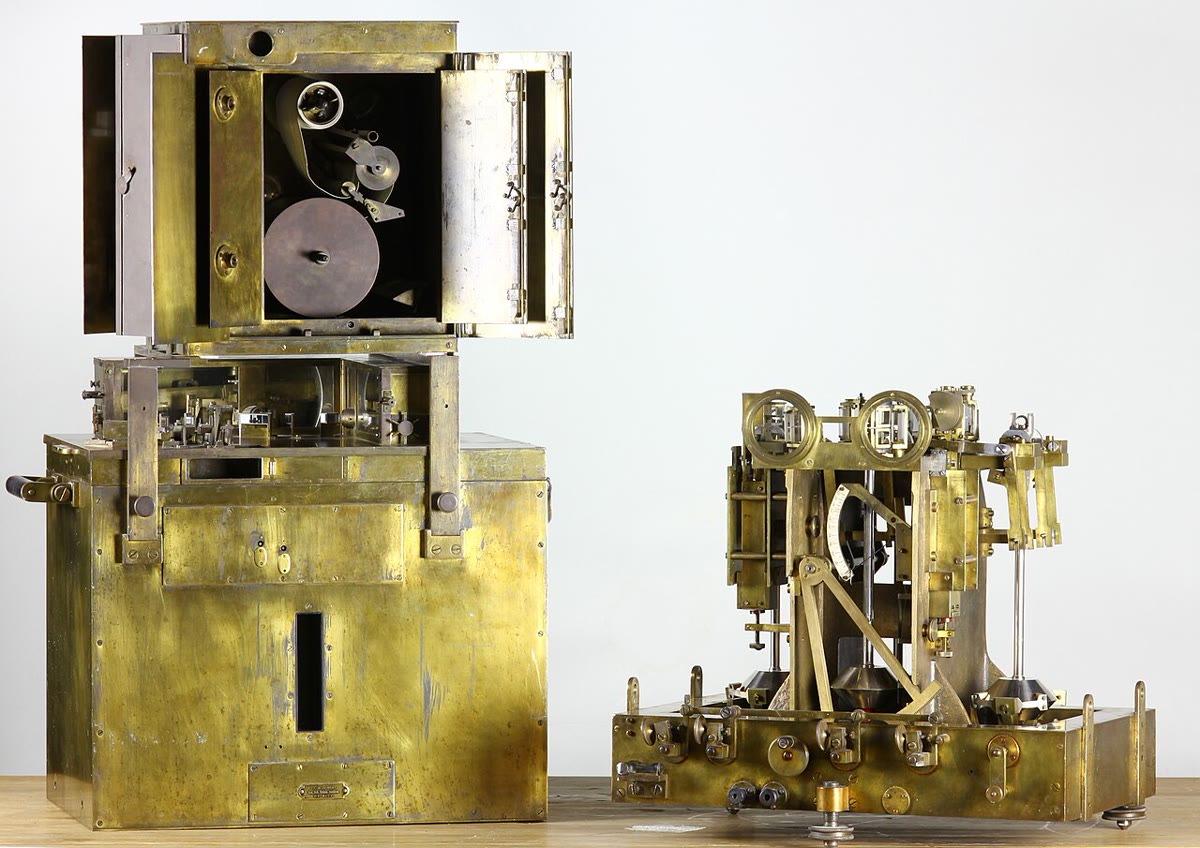
\includegraphics[width=\linewidth]{images/book3/b1-vening-meinesz.jpg}

{\scriptsize Sebuah peralatan bandul Vening Meinesz (kanan) dan kotaknya dengan unit perekam (Broodt, CC BY-SA 4.0).}
\end{minipage}
\end{history}

\section{Geoid}

Permukaan laut dalam keadaan diam adalah permukaan potensial gravitasi yang konstan: jika tidak, air akan mengalir di sepanjangnya. Ia adalah acuan alami untuk ketinggian, dan permukaan tempat tali unting lama tegak lurus.

\begin{definition}[Geoid; tinggi geoid]\label{def:b1:isostasy-gravity:geoid}
\emph{Geoid}\index{geoid} adalah permukaan ekuipotensial gravitasi Bumi (gravitasi ditambah efek sentrifugal rotasi) yang berimpit dengan permukaan laut rata-rata di samudra terbuka, dalam keadaan diam, dan dilanjutkan di bawah benua. \emph{Tinggi geoid}\index{tinggi geoid} $N$ di suatu titik adalah tinggi geoid di atas elipsoid acuan, dihitung negatif di tempat geoid berada di bawahnya.
\end{definition}

Ketinggian di atas permukaan laut pada peta adalah ketinggian di atas \omterm{def:b1:isostasy-gravity:geoid}{geoid}; ketinggian yang diberikan oleh penentuan posisi satelit adalah ketinggian di atas elipsoid; keduanya berbeda sebesar $N$. \omterm{def:b1:isostasy-gravity:geoid}{Geoid} menyimpang dari elipsoid sebesar \qty{+85}{m} di dekat Islandia dan \qty{-106}{m} di lepas India selatan, kurang dari \qty{200}{m} seluruhnya, sedangkan relief permukaan padat membentang sekitar \qty{20}{km}: \omterm{def:b1:isostasy-gravity:geoid}{geoid} adalah permukaan yang jauh lebih halus daripada tanah.
% ledger: nasa:geoid-range, earth:topo

\begin{proposition}[Tinggi geoid dan anomali potensial]\label{prop:b1:isostasy-gravity:bruns}
Misalkan $\Phi$ potensial gravitasi Bumi dan $\Phi_n$ potensial normal, yaitu milik model Bumi yang permukaannya, elipsoid acuan, memiliki potensial yang sama $\Phi_0$ dengan \omterm{def:b1:isostasy-gravity:geoid}{geoid}, keduanya dihitung dengan tanda fisika (potensial naik ke atas dan $g = -\nabla\Phi$). Misalkan $T = \Phi - \Phi_n$ adalah anomali potensial di \omterm{def:b1:isostasy-gravity:geoid}{geoid}. Hingga orde pertama,
\[
  N = -\frac{T}{\gamma} .
\]
Ahli geodesi, yang menghitung potensial dengan tanda sebaliknya, menulis hasil yang sama $N = T/\gamma$, rumus Bruns.
\end{proposition}

\begin{proof}
Misalkan $Q$ titik pada elipsoid dan $P$ titik pada \omterm{def:b1:isostasy-gravity:geoid}{geoid} di sepanjang normal melalui $Q$, pada ketinggian $N$. Potensial normal naik ke atas
dengan laju $\gamma$, sehingga $\Phi_n(P) \approx \Phi_n(Q) + \gamma N = \Phi_0 +
\gamma N$. Karena $P$ berada pada \omterm{def:b1:isostasy-gravity:geoid}{geoid}, $\Phi(P) = \Phi_0$, yaitu
$\Phi_n(P) + T = \Phi_0$. Maka $\Phi_0 + \gamma N + T = \Phi_0$ dan $N =
-T/\gamma$.
\end{proof}

Kelebihan massa di bawah suatu titik membuat potensial di sana lebih negatif, sehingga $T < 0$ dan $N > 0$: \omterm{def:b1:isostasy-gravity:geoid}{geoid} menggembung ke atas di atas kelebihan massa dan tenggelam di atas defisit. Tinggi \qty{85}{m} di dekat Islandia berkorespondensi dengan anomali potensial sebesar $-\qty{85}{m}\times\qty{9.8}{m.s^{-2}} \approx \qty{-830}{J.kg^{-1}}$.
Karena potensial meluruh sebagai $1/r$ sedangkan tarikan meluruh sebagai $1/r^2$, \omterm{def:b1:isostasy-gravity:geoid}{geoid} didominasi oleh massa besar dan dalam, dan \omterm{def:b1:isostasy-gravity:anomalies}{anomali gravitasi} oleh massa yang dangkal. Pegunungan yang terkompensasi hanya sedikit menaikkan \omterm{def:b1:isostasy-gravity:geoid}{geoid}, karena kelebihan massanya dan defisit akarnya hampir saling meniadakan; beban yang tidak terkompensasi menaikkannya jauh lebih banyak.

\begin{omfigure}
\begin{tikzpicture}[x=1.15cm, y=1.3cm, font=\scriptsize, >={Stealth[length=4pt]}]
% schematic, not to scale
\fill[omSea!35] (0,0.05) .. controls (1.5,0.25) and (2.5,0.35) .. (3.6,0.45) -- (3.6,-1.2) -- (0,-1.2) -- cycle;
\fill[omLithGranite!40] (3.6,0.45) .. controls (4.5,1.4) and (5.4,1.9) .. (6.4,1.7) .. controls (7.4,1.5) and (8.2,1.2) .. (9,1.0) -- (9,-1.2) -- (3.6,-1.2) -- cycle;
\fill[omLithGabbro!35] (0,-0.7) .. controls (1.2,-0.9) and (2.4,-0.6) .. (3.6,-0.2) -- (3.6,-1.2) -- (0,-1.2) -- cycle;
\draw[thick, blue!70!black] (0,0.05) .. controls (1.5,0.25) and (2.5,0.35) .. (3.6,0.45) .. controls (5,0.75) and (7,0.75) .. (9,0.55);
\draw[thick, black, densely dashed] (0,-0.25) .. controls (3,0.05) and (6,0.15) .. (9,0.1);
\draw (3.6,0.45) .. controls (4.5,1.4) and (5.4,1.9) .. (6.4,1.7) .. controls (7.4,1.5) and (8.2,1.2) .. (9,1.0);
\node[anchor=west, blue!70!black] at (9.05,0.6) {geoid};
\node[anchor=west] at (9.05,0.1) {elipsoid};
\node[anchor=west] at (9.05,1.0) {tanah};
\node at (1.4,-0.3) {samudra};
\node at (1.6,-1.0) {dasar laut};
% heights (curve ordinates computed from the Bezier segments)
\draw[<->] (6.6,0.107) -- (6.6,0.688); \node[anchor=east] at (6.57,0.40) {$N$};
\draw[<->] (7.2,0.674) -- (7.2,1.512); \node[anchor=west] at (7.23,1.09) {$H$};
\draw[<->] (8.2,0.110) -- (8.2,1.224); \node[anchor=east] at (8.17,0.95) {$h_e$};
% the vertical (perpendicular to the geoid) and the ellipsoid normal at x = 2.4 (angle exaggerated)
\draw[->, thick, blue!70!black] (2.4,0.335) -- (2.0,1.3);
\draw[->, thick, black] (2.4,0.335) -- (2.33,1.3);
\node[anchor=south east, blue!70!black] at (2.05,1.3) {vertikal (tali unting)};
\node[anchor=south west] at (2.3,1.3) {normal elipsoid};
\end{tikzpicture}

\par\smallskip{\small \omterm{def:b1:isostasy-gravity:geoid}{Geoid} (biru), elipsoid acuan (putus-putus) dan tanah (skematis; penyimpangan sangat dibesar-besarkan). Di atas samudra \omterm{def:b1:isostasy-gravity:geoid}{geoid} adalah permukaan laut dalam keadaan diam; di bawah daratan ia dilanjutkan sebagai ekuipotensial. Tinggi $H$ pada peta diukur dari \omterm{def:b1:isostasy-gravity:geoid}{geoid}, tinggi $h_e$ yang diberikan oleh penentuan posisi satelit dari elipsoid, dan $h_e = H + N$. Tali unting tegak lurus terhadap \omterm{def:b1:isostasy-gravity:geoid}{geoid}, bukan terhadap elipsoid: sudut di antara keduanya (dibesar-besarkan di sini) adalah defleksi vertikal yang mengganggu para juru ukur India.}
\label{fig:b1:isostasy-gravity:geoid}
\end{omfigure}

Defleksinya kecil: seluruh selisih yang mengganggu para juru ukur India hanya sekitar lima detik busur. Di atas samudra \omterm{def:b1:isostasy-gravity:geoid}{geoid} dapat terlihat.
Sejak 1978, altimeter radar pada satelit telah mengukur waktu denyut gelombang mikro yang dipantulkan dari permukaan laut untuk mengukur tingginya. Setelah pasang surut, gelombang dan arus dirata-ratakan, permukaan laut berdiri lebih tinggi di atas gunung laut dan punggungan, dan lebih rendah di atas palung dan dataran abisal, dan tonjolan-tonjolan ini (\cref{exo:b1:isostasy-gravity:11} memperkirakan satu) memetakan topografi dasar laut dalam di tempat tidak ada kapal yang menyelam. Satelit GOCE, dari 2009 hingga 2013, terbang pada sekitar \qty{260}{km} dan mengukur medan gravitasi dari orbit, dengan sasaran \omterm{def:b1:isostasy-gravity:geoid}{geoid} hingga 1 hingga
\qty{2}{cm} dan \omterm{def:b1:isostasy-gravity:anomalies}{anomali gravitasi} hingga sekitar \qty{1}{\milli\gal}, dengan resolusi lebih baik daripada \qty{100}{km}.
% ledger: pratt:himalaya, jpl:seasat, esa:goce

\subsection*{Isostasi yang bergerak}

\omterm{def:b1:isostasy-gravity:isostasy}{Isostasi} dicapai dengan aliran, dan aliran membutuhkan waktu. Pada puncak glasiasi terakhir, sekitar \num{20000} tahun yang lalu, lapisan es setebal sekitar \qty{3}{km} menutupi Skandinavia.
Es memiliki massa jenis sekitar sembilan persepuluh air, sehingga dengan \omterm{def:b1:layered-earth:layers}{mantel} \qty{3300}{kg.m^{-3}}, depresi isostatik penuh di bawah lapisan es seperti itu adalah
$\qty{3000}{m}\times900/3300 \approx \qty{820}{m}$. Es telah hilang, dan daratan masih naik: penentuan posisi satelit mengukur hingga sekitar \qty{10}{mm.yr^{-1}} pengangkatan di Swedia utara, di sebelah barat Teluk Bothnia, hari ini. Laju
tempat depresi itu mengendur mengukur viskositas \omterm{def:b1:layered-earth:layers}{mantel} di bawahnya, pokok bahasan volume Sarjana Tahun ke-3; \cref{exo:b1:isostasy-gravity:12} menunjukkan caranya.
% ledger: kierulf:fennoscandia, usgs:ice-density

\section{Latihan}

\begin{exercise}[$\star$]\label{exo:b1:isostasy-gravity:1}
(a) Ubah \omterm{def:b1:isostasy-gravity:anomalies}{anomali Bouguer} \qty{-150}{\milli\gal} ke \unit{m.s^{-2}}, dan nyatakan sebagai fraksi dari $g = \qty{9.81}{m.s^{-2}}$. (b) Sama untuk \qty{1}{\milli\gal}, presisi yang ditargetkan untuk \omterm{def:b1:isostasy-gravity:anomalies}{anomali gravitasi} dari GOCE, dan untuk \qty{1}{\micro\gal}.
% ledger: esa:goce, nist:gal
\end{exercise}

\begin{exercise}[$\star$]\label{exo:b1:isostasy-gravity:2}
(a) Hitung \omterm{def:b1:isostasy-gravity:normal-gravity}{gravitasi normal} di ekuator, pada \ang{45} dan di kutub dengan rumus dalam bab ini. (b) Berikan selisih ekuator-kutub dalam miligal. (c) Percepatan sentrifugal di ekuator adalah \qty{3392}{\milli\gal}. Berapa fraksi selisih itu yang dijelaskan rotasi secara langsung?
% ledger: moritz:grs80
\end{exercise}

\begin{exercise}[$\star$]\label{exo:b1:isostasy-gravity:3}
Sebuah dataran tinggi berdiri \qty{3}{km} di atas permukaan laut. Dengan \omterm{def:b1:layered-earth:layers}{kerak} bermassa jenis \qty{2800}{kg.m^{-3}} dan \omterm{def:b1:layered-earth:layers}{mantel} \qty{3300}{kg.m^{-3}}, hitung akar Airy-nya dan penebalan \omterm{def:b1:layered-earth:layers}{keraknya}.
\end{exercise}

\begin{exercise}[$\star$]\label{exo:b1:isostasy-gravity:4}
(a) Sebesar apa gravimeter harus dinaikkan agar pembacaannya turun sebesar \qty{1}{\milli\gal}? Gunakan \qty{0.3086}{\milli\gal.m^{-1}}. (b) Sebuah survei menargetkan anomali hingga \qty{0.01}{\milli\gal}. Sampai ketelitian berapa ketinggian stasiun harus diketahui?
\end{exercise}

\begin{exercise}[$\star\star$]\label{exo:b1:isostasy-gravity:5}
Dalam model Pratt dengan $D = \qty{100}{km}$ dan $\rho_0 = \qty{2700}{kg.m^{-3}}$, (a) hitung massa jenis kolom-kolom yang berdiri setinggi 1, 3 dan \qty{5}{km}; (b) hitung massa jenis kolom di bawah \qty{4}{km} air laut bermassa jenis \qty{1030}{kg.m^{-3}}. (c) Mengapa model Pratt lebih cocok untuk dasar laut daripada untuk benua?
\end{exercise}

\begin{exercise}[$\star\star$]\label{exo:b1:isostasy-gravity:6}
Dua stasiun berada pada \omterm{def:b1:spherical-astronomy:geographic}{lintang} \ang{48}, tempat \omterm{def:b1:isostasy-gravity:normal-gravity}{gravitasi normal} adalah \qty{9.808911}{m.s^{-2}}. Stasiun 1, \qty{350}{m} di atas permukaan laut, membaca \qty{9.807751}{m.s^{-2}}; stasiun 2, pada \qty{1850}{m}, membaca \qty{9.803552}{m.s^{-2}}. (a) Hitung \omterm{def:b1:isostasy-gravity:anomalies}{anomali udara-bebas} dan Bouguer keduanya, dengan massa jenis Bouguer standar. (b) Apa yang disarankan anomali stasiun 2 tentang pegunungan di sekitarnya?
\end{exercise}

\begin{exercise}[$\star\star$]\label{exo:b1:isostasy-gravity:7}
(a) Dengan mengikuti pembuktian \cref{prop:b1:isostasy-gravity:slab}, tunjukkan bahwa cakram horizontal berjari-jari $a$, tebal $h$ dan massa jenis $\rho$ menarik titik pada sumbunya,
pada jarak $z \gg h$ di atasnya, dengan $2\pi G\rho h\,\bigl(1 -
z/\sqrt{z^2 + a^2}\bigr)$. (b) Jari-jari berapa yang memberikan \qty{90}{\percent} dari nilai lempeng pada $z = \qty{1}{km}$? (c) Apa yang dikatakan ini tentang luas medan yang berpengaruh pada \omterm{def:b1:isostasy-gravity:anomalies}{koreksi Bouguer}?
\end{exercise}

\begin{exercise}[$\star\star$]\label{exo:b1:isostasy-gravity:8}
Dalam model Airy dengan \omterm{def:b1:layered-earth:layers}{kerak} \qty{2800}{kg.m^{-3}}, setebal \qty{35}{km} di permukaan laut, di atas \omterm{def:b1:layered-earth:layers}{mantel} \qty{3300}{kg.m^{-3}}, (a) hitung anti-akar dan ketebalan \omterm{def:b1:layered-earth:layers}{kerak} di bawah \qty{4}{km} air laut dengan massa jenis \qty{1030}{kg.m^{-3}}.
(b) \omterm{def:b1:layered-earth:layers}{Kerak} samudra sebenarnya sekitar \qty{5}{km} tebalnya. Apa yang ditunjukkan oleh selisih itu? % ledger: usgs:crust-thickness
\end{exercise}

\begin{exercise}[$\star\star$]\label{exo:b1:isostasy-gravity:9}
Dalam uraian pembukaan, selisih \omterm{def:b1:spherical-astronomy:geographic}{lintang} antara Kaliana dan Kalianpur adalah \qty{5.236}{''}, sedangkan tarikan Himalaya yang dihitung Pratt seharusnya menghasilkan \qty{15.885}{''}. (a) Ubah kedua sudut menjadi radian.
(b) Percepatan horizontal $a_h$ memiringkan tali unting sebesar sudut $a_h/g$. Selisih tarikan horizontal antara kedua
stasiun yang sesuai dengan masing-masing sudut itu, dalam miligal, dengan
$g = \qty{9.79}{m.s^{-2}}$? (c) Berapa fraksi tarikan pegunungan yang terlihat yang dibatalkan oleh kompensasi?
% ledger: pratt:himalaya
\end{exercise}

\begin{exercise}[$\star\star\star$]\label{exo:b1:isostasy-gravity:10}
Sebuah kubah garam dimodelkan sebagai bola berjari-jari \qty{2}{km}, dengan pusatnya pada kedalaman \qty{4}{km} dan massa jenis \qty{200}{kg.m^{-3}} lebih rendah daripada batuan di sekitarnya. (a) Tunjukkan bahwa bola terpendam dengan massa anomali $M$ pada kedalaman $z$
memberikan, pada jarak horizontal $x$, anomali $GMz/(x^2 + z^2)^{3/2}$. (b) Hitung anomali di atas pusatnya. (c) Pada jarak berapa anomali itu turun menjadi setengah nilai puncaknya? (d) Bagaimana kedalaman sebuah bola dapat dibaca dari profil terukur?
\end{exercise}

\begin{exercise}[$\star\star\star$]\label{exo:b1:isostasy-gravity:11}
Sebuah gunung laut adalah kerucut setinggi \qty{3}{km} dengan alas berjari-jari \qty{15}{km} yang berdiri di atas dasar laut sedalam \qty{5}{km}. Batuannya bermassa jenis \qty{2800}{kg.m^{-3}}, air laut \qty{1030}{kg.m^{-3}}. (a) Hitung kelebihan massanya atas air yang dipindahkannya. (b) Anggap ia sebagai massa titik di pusat massanya, seperempat tingginya di atas alas, dan gunakan
\cref{prop:b1:isostasy-gravity:bruns} dengan $\gamma = \qty{9.81}{m.s^{-2}}$ untuk memperkirakan tinggi tonjolan permukaan laut di atasnya. (c) Apakah massa titik melebih-lebihkan atau meremehkan tonjolan itu? (d) Jika gunung laut itu sepenuhnya dikompensasi oleh akar, bagaimana tonjolan itu berubah?
\end{exercise}

\begin{exercise}[$\star\star\star$]\label{exo:b1:isostasy-gravity:12}
Modelkan pemulihan Skandinavia setelah es mencair: anggap es lenyap mendadak \num{10000} tahun yang lalu, meninggalkan depresi sebesar \qty{818}{m} yang sejak itu berkurang sebagai $w(t) = w_0\,e^{-t/\tau}$. (a) Tunjukkan bahwa laju pengangkatannya adalah
$w/\tau$. (b) Dengan $\tau = \num{4000}$ tahun, hitung depresi yang tersisa dan laju pengangkatan hari ini, dan bandingkan laju itu dengan \qty{10}{mm.yr^{-1}} yang terukur. (c) Tunjukkan bahwa $\tau = \num{3100}$ tahun dan $\tau = \num{68000}$ tahun keduanya memberikan sekitar \qty{10}{mm.yr^{-1}} hari ini. Depresi tersisa apa yang disiratkan masing-masing, dan bagaimana survei gravitasi dapat memutuskan di antara keduanya? (d) Sifat \omterm{def:b1:layered-earth:layers}{mantel} apa yang diukur oleh $\tau$?
% ledger: kierulf:fennoscandia
\end{exercise}

\section{Soal: akar suatu pegunungan}

\begin{problem}[{Soal akhir pekan --- akar suatu dataran tinggi, Airy melawan Pratt, gravitasi di atasnya, dan apa yang dilakukan erosi kepadanya}]
\label{pb:b1:isostasy-gravity:1}
% values: calc/ch11.py (invented plateau; normal gravity formula of the chapter)
% ledger: moritz:grs80, usgs73:reduction
Sebuah dataran tinggi yang luas, beberapa ratus kilometer lebarnya, berdiri \qty{4}{km} di atas dataran rendah di permukaan laut yang \omterm{def:b1:layered-earth:layers}{keraknya} setebal \qty{35}{km}. Ambil $\rho_c = \qty{2700}{kg.m^{-3}}$ untuk \omterm{def:b1:layered-earth:layers}{kerak}, $\rho_m = \qty{3300}{kg.m^{-3}}$ untuk \omterm{def:b1:layered-earth:layers}{mantel}, $g = \qty{9.81}{m.s^{-2}}$, dan $2\pi G = \qty{0.0419}{\milli\gal}$ per meter per \qty{1000}{kg.m^{-3}}.

\medskip
\noindent\textbf{Bagian I --- Dataran tinggi Airy.}
\begin{enumerate}
  \item Hitung akar Airy dari dataran tinggi itu.
  \item Turunkan ketebalan \omterm{def:b1:layered-earth:layers}{keraknya} dan kedalaman \omterm{def:b1:layered-earth:discontinuity}{Moho-nya} di bawah permukaan laut.
  \item Ambil \omterm{def:b1:isostasy-gravity:isostasy}{kedalaman kompensasi} pada \qty{60}{km} di bawah permukaan laut. Hitung massa per meter persegi di atasnya pada kolom dataran tinggi dan pada kolom dataran rendah.
  \item Hitung tekanan pada kedalaman \qty{60}{km}.
  \item Mengapa akar itu 4.5 kali ketinggiannya? Berapa rasionya dengan \omterm{def:b1:layered-earth:layers}{kerak} bermassa jenis \qty{2900}{kg.m^{-3}}?
  \item Apa yang akan ditunjukkan oleh survei refraksi seismik melintasi tepi dataran tinggi jika model Airy berlaku?
\end{enumerate}

\noindent\textbf{Bagian II --- Dataran tinggi Pratt.}
Sekarang misalkan sebaliknya \omterm{def:b1:isostasy-gravity:isostasy}{kedalaman kompensasi} $D = \qty{100}{km}$ di bawah permukaan laut dan sebuah kolom dataran rendah dengan massa jenis seragam \qty{2700}{kg.m^{-3}}.
\begin{enumerate}[resume]
  \item Hitung massa jenis kolom dataran tinggi.
  \item Periksa bahwa kedua kolom memiliki massa per meter persegi yang sama di atas $D$.
  \item Berapa persen kolom dataran tinggi harus lebih ringan?
  \item Jika selisih massa jenis ini hanya disebabkan oleh panas, dengan koefisien ekspansi termal \qty{3e-5}{K^{-1}}, berapa banyak lebih panaskah kolom dataran tinggi rata-rata? Apakah itu masuk akal?
  \item Di mana \omterm{def:b1:layered-earth:discontinuity}{Moho} di bawah dataran tinggi dalam model Pratt?
  \item Survei refraksi mendapati \omterm{def:b1:layered-earth:discontinuity}{Moho} pada \qty{52}{km} di bawah dataran tinggi. Model mana yang cocok?
\end{enumerate}

\noindent\textbf{Bagian III --- Gravitasi di atas pusat.}
\begin{enumerate}[resume]
  \item Hitung \omterm{def:b1:isostasy-gravity:anomalies}{koreksi Bouguer} untuk stasiun di atas dataran tinggi.
  \item Prediksikan \omterm{def:b1:isostasy-gravity:anomalies}{anomali udara-bebas} dan Bouguer di pusat jika dataran tinggi itu tidak dikompensasi.
  \item Prediksikan keduanya untuk dataran tinggi Airy, dan periksa \omterm{def:b1:isostasy-gravity:anomalies}{anomali Bouguer} dengan massa yang hilang dari akar itu.
  \item Sebuah stasiun di pusat dataran tinggi, pada \omterm{def:b1:spherical-astronomy:geographic}{lintang} \ang{30} dan \qty{4000}{m}, membaca \qty{9.781085}{m.s^{-2}}. Hitung \omterm{def:b1:isostasy-gravity:normal-gravity}{gravitasi normal} pada \ang{30}, lalu \omterm{def:b1:isostasy-gravity:anomalies}{anomali udara-bebas} dan Bouguer.
  \item Berapa fraksi dataran tinggi yang terkompensasi?
  \item Apakah \omterm{def:b1:isostasy-gravity:anomalies}{anomali Bouguer} di pusat akan berbeda jika dataran tinggi itu dikompensasi dengan cara Pratt? Jelaskan.
  \item Sketsakan \omterm{def:b1:isostasy-gravity:anomalies}{anomali udara-bebas} sepanjang profil melintasi salah satu tepi dataran tinggi, dan jelaskan bentuknya.
\end{enumerate}

\noindent\textbf{Bagian IV --- Erosi.}
Sungai mengangkut lapisan setebal \qty{1}{km} dari seluruh permukaan dataran tinggi, cukup lambat agar \omterm{def:b1:isostasy-gravity:isostasy}{isostasi} dapat mengikuti.
\begin{enumerate}[resume]
  \item Berapa ketebalan \omterm{def:b1:layered-earth:layers}{kerak} yang baru, dan berapa akar Airy barunya?
  \item Berapa ketinggian baru dataran tinggi itu?
  \item Berapa banyak batuan yang kini berada di permukaan telah naik?
  \item Berapa banyak batuan yang harus dierosi seluruhnya untuk menurunkan dataran tinggi ke permukaan laut? Apa yang ini katakan tentang batuan yang terlihat di sabuk gunung tua?
  \item Berapa banyak permukaan dataran tinggi turun untuk setiap kilometer batuan yang dierosi?
\end{enumerate}
\end{problem}
